% Options for packages loaded elsewhere
\PassOptionsToPackage{unicode}{hyperref}
\PassOptionsToPackage{hyphens}{url}
%
\documentclass[
]{article}
\usepackage{lmodern}
\usepackage{amssymb,amsmath}
\usepackage{ifxetex,ifluatex}
\ifnum 0\ifxetex 1\fi\ifluatex 1\fi=0 % if pdftex
  \usepackage[T1]{fontenc}
  \usepackage[utf8]{inputenc}
  \usepackage{textcomp} % provide euro and other symbols
\else % if luatex or xetex
  \usepackage{unicode-math}
  \defaultfontfeatures{Scale=MatchLowercase}
  \defaultfontfeatures[\rmfamily]{Ligatures=TeX,Scale=1}
\fi
% Use upquote if available, for straight quotes in verbatim environments
\IfFileExists{upquote.sty}{\usepackage{upquote}}{}
\IfFileExists{microtype.sty}{% use microtype if available
  \usepackage[]{microtype}
  \UseMicrotypeSet[protrusion]{basicmath} % disable protrusion for tt fonts
}{}
\makeatletter
\@ifundefined{KOMAClassName}{% if non-KOMA class
  \IfFileExists{parskip.sty}{%
    \usepackage{parskip}
  }{% else
    \setlength{\parindent}{0pt}
    \setlength{\parskip}{6pt plus 2pt minus 1pt}}
}{% if KOMA class
  \KOMAoptions{parskip=half}}
\makeatother
\usepackage{xcolor}
\IfFileExists{xurl.sty}{\usepackage{xurl}}{} % add URL line breaks if available
\IfFileExists{bookmark.sty}{\usepackage{bookmark}}{\usepackage{hyperref}}
\hypersetup{
  pdftitle={10 - Reproducibility},
  pdfauthor={Kevin Lanning},
  hidelinks,
  pdfcreator={LaTeX via pandoc}}
\urlstyle{same} % disable monospaced font for URLs
\usepackage[margin=1in]{geometry}
\usepackage{graphicx}
\makeatletter
\def\maxwidth{\ifdim\Gin@nat@width>\linewidth\linewidth\else\Gin@nat@width\fi}
\def\maxheight{\ifdim\Gin@nat@height>\textheight\textheight\else\Gin@nat@height\fi}
\makeatother
% Scale images if necessary, so that they will not overflow the page
% margins by default, and it is still possible to overwrite the defaults
% using explicit options in \includegraphics[width, height, ...]{}
\setkeys{Gin}{width=\maxwidth,height=\maxheight,keepaspectratio}
% Set default figure placement to htbp
\makeatletter
\def\fps@figure{htbp}
\makeatother
\usepackage[normalem]{ulem}
% Avoid problems with \sout in headers with hyperref
\pdfstringdefDisableCommands{\renewcommand{\sout}{}}
\setlength{\emergencystretch}{3em} % prevent overfull lines
\providecommand{\tightlist}{%
  \setlength{\itemsep}{0pt}\setlength{\parskip}{0pt}}
\setcounter{secnumdepth}{-\maxdimen} % remove section numbering
\ifluatex
  \usepackage{selnolig}  % disable illegal ligatures
\fi

\title{10 - Reproducibility}
\author{Kevin Lanning}
\date{2021-02-07}

\begin{document}
\maketitle

\hypertarget{reproducibility-and-the-replication-crisis}{%
\section{Reproducibility and the replication
crisis}\label{reproducibility-and-the-replication-crisis}}

Probability theory is elegant, and the logic of \textbf{Null Hypothesis
Significance Testing (NHST)} is compelling. But philosophers of science
have long recognized that this is not really how science works
{[}@lakatos1969{]}. That is, science is not primarily built by the
testing and rejecting of null hypotheses. (Think, for example, of how
you might describe an experiment for testing the hypothesis that gravity
exists, and whether you would ever reject this hypothesis).

The problem is a multifaceted one. It arises partly because, in any
experiment, there is a large (infinite?) number of conditions which
might be invoked to explain-away results of a failure of our work. It
arises because we are human, and prone to various biases of decision
making and information integration (that is, we are poor Bayesians). It
arises, too, because scientific institutions such as journals, funding
agencies, and universities are competitive environments which
incentivize positive findings.

In recent years, the tension between \textbf{the false ideal of NHST}
and the real world of science has become increasingly evident. Within
psychology, experimental studies have often - even typically - failed to
replicate well-known results {[}@open2015{]}. It's not just psychology
{[}@baker2016{]}. One of the first important papers to shine light in
the area {[}@ioannidis2005{]} came from medicine; it suggested six
contributing factors, which I quote verbatim here:

\begin{quote}
\emph{The smaller the studies conducted in a scientific field, the less
likely the research findings are to be true.}

\begin{itemize}
\tightlist
\item
  This stems directly from our discussion of the central limit theorem
  and the instability of results from small samples.
\end{itemize}

\emph{The smaller the effect sizes in a scientific field, the less
likely the research findings are to be true}

\begin{itemize}
\tightlist
\item
  We'll talk about effect size below.
\end{itemize}

\emph{The greater the number and the lesser the selection of tested
relationships in a scientific field, the less likely the research
findings are to be true.} (and) \emph{The greater the flexibility in
designs, definitions, outcomes, and analytical modes in a scientific
field, the less likely the research findings are to be true.}

\begin{itemize}
\tightlist
\item
  The ``problem'' of analytic flexibility leads to `p-hacking'
\end{itemize}

\emph{The greater the financial and other interests and prejudices in a
scientific field, the less likely the research findings are to be true}
and \emph{The hotter a scientific field (with more scientific teams
involved), the less likely the research findings are to be true.}

\begin{itemize}
\tightlist
\item
  Positive findings rise, and negative ones are ignored. And scientists
  are human, and subject to incentives.
\end{itemize}
\end{quote}

Here's a video which provides some more context for the crisis:

\href{https://youtu.be/42QuXLucH3Q}{\includegraphics{https://img.youtube.com/vi/42QuXLucH3Q/0.jpg}}.

*Video 10.1: On the reproducibility crisis (12 mins)

\hypertarget{answers-to-the-reproducibility-crisis}{%
\subsection{Answers to the reproducibility
crisis}\label{answers-to-the-reproducibility-crisis}}

For scientific progress to occur, there needs to be more than a simple
rejection of what is wrong with current methods and research programs:
Here, as elsewhere, criticism must be constructive to be valuable.

There have been a number of solutions proposed to the reproducibility
crisis.

\hypertarget{tweak-or-abandon-nhst}{%
\subsubsection{Tweak or abandon NHST}\label{tweak-or-abandon-nhst}}

The first cluster of responses to the reproducibility crisis is
concerned with statistics, specifically problems with Null Hypothesis
Significance Testing (NHST). These include (a) justifying one's alpha -
making it more stringent, for example, for counter-intuitive claims
{[}@grange2018{]}, (b) changing the default p value from .05 to .005
{[}@benjamin2017{]}, and (c) abandoning significance testing altogether
{[}@mcshane2017{]}.

@szucs2017 goes into some of these issues in more detail and discusses
other limitations of significance testing, including the dichotomous,
all-or-none silliness of the accept/reject decision. (If you play the
NHST game, there is no `almost' significant, `approached significance,'
`highly significant', etc.).

@leek2015 argue that the problems are not merely with NHST, but with the
whole of data analysis. They maintain that better training in data
science - courses like ours, perhaps, are part of the answer.

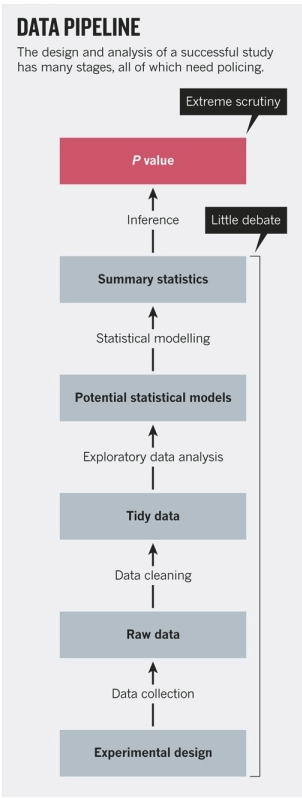
\includegraphics{images/leek2015pipeline.PNG} (figure)

@munafo2017 also argue that threats to reproducible science occur at a
number of places in science, not just with the evaluation of hypotheses.

\begin{figure}
\centering
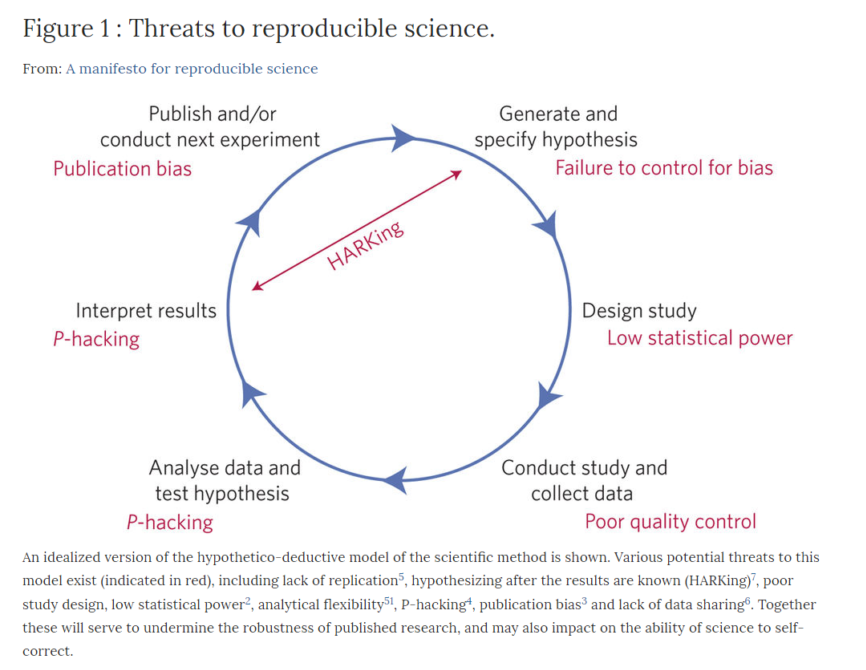
\includegraphics{images/munafo2017threats.PNG}
\caption{munafo2017threats}
\end{figure}

\hypertarget{keep-a-log-of-every-step-of-every-analysis-in-r-markdown-or-jupyter-notebooks}{%
\subsubsection{Keep a log of every step of every analysis in R markdown
or Jupyter
notebooks}\label{keep-a-log-of-every-step-of-every-analysis-in-r-markdown-or-jupyter-notebooks}}

A second cluster of responses is concerned with keeping good records.
Let's say that you are running a study, say, which looks at the
hypothesis of differential variation of females and males in a cognitive
measure; your interest is to critically examine the hypothesis discussed
by @wainer2007 that males show more variability.

There have been \emph{a lot} of studies related to this over the years,
so that rather than collect new data you decide that you will work with
existing data from several online archives. You find and download
spreadsheets from two studies: In the first, gender is coded `1' for
male, `2' for female. In the second, gender is coded `1' for female, `2'
for male, and `3' for other. There are, in essence, two ways that you
can combine the variables into a common format: The first would be to
take one of the spreadsheets and do a few find-and-replace commands on
the appropriate column of the data. This is quick and easy - but when
someone else, or even future you, returns to this data, you will not
remember if you have recoded it.

The alternative is to keep a record of your work in R markdown. This is
more time consuming, and can sometimes be clumsy. But it is
\sout{virtuous} useful and clear - and when you screw up, you will have
a full record of what happened.

Part of the problem of scientific reproducibility is to keep
comprehensive records. This record-keeping and research transparency is
at the heart of R markdown documents.

\hypertarget{answers-to-the-reproducibility-crisis-iii-pre-registration}{%
\subsection{Answers to the reproducibility crisis III:
Pre-registration}\label{answers-to-the-reproducibility-crisis-iii-pre-registration}}

The third answer to the reproducibility crisis is the most
comprehensive; it involves not merely keeping a record of what you have
done, but preregistering your work, that is, fully specifying your
planned analyses beforehand {[}@miguel2014{]}. The author, an economist,
outlines his argument in a five-minute video
\href{https://www.futurelearn.com/courses/open-social-science-research/0/steps/31436}{here}.
For randomized controlled trials, consider socialscienceregistry.org,
and for more general use, use the open science framework page.

\hypertarget{further-readings}{%
\subsection{Further readings}\label{further-readings}}

Finally, if you would like to learn more about the reproducibility
crisis, there is a collection of papers in Nature
\href{https://www.nature.com/collections/prbfkwmwvz/}{here}.

\end{document}
